\documentclass[11pt]{article}
\usepackage[margin=1in]{geometry}
\usepackage{amsmath,amssymb,amsthm}
\usepackage{booktabs}
\usepackage{graphicx}
\usepackage[colorlinks=true,linkcolor=blue,citecolor=blue,urlcolor=blue]{hyperref}
\newcommand{\ueV}{\,\mu\mathrm{eV}}
\newcommand{\nx}{\nu_x}\newcommand{\ny}{\nu_y}\newcommand{\nz}{\nu_z}
\newtheorem{theorem}{Theorem}
\newtheorem{proposition}{Proposition}
\title{Supplementary Material:\\ Majorana zero modes in silicon}
\author{W.~T.~Trevena}
\date{June 2026 --- accompanies draft v2}
\begin{document}
\maketitle
\tableofcontents

\section{Model, basis, and the physical pairing channel}\label{s:model}
\subsection{Single-channel BdG conventions}
The normal-state Hamiltonian on $N$ sites with spacing $dx$ is
\begin{equation}
h = \sum_n c_n^\dagger\!\left[(2t-\mu+V_n)\sigma_0 + E_Z\sigma_x\right]\!c_n
+ \sum_n \left[c_{n+1}^\dagger\!\left(-t\sigma_0 - i\,a_{so}\sigma_z\right)\!c_n
+ \mathrm{h.c.}\right],
\end{equation}
with $t=\hbar^2/2m^* dx^2$, $a_{so}=\alpha/2dx$, $E_Z=\tfrac12 g\mu_B B$, and
singlet pairing $\Delta\, i\sigma_y$. The BdG matrix is assembled as
$H=\begin{pmatrix} h & D\\ D^\dagger & -h^*\end{pmatrix}$,
$D = \Delta\,\mathbb{1}_N\otimes i\sigma_y$, which enforces particle--hole
symmetry $\mathcal{P}=\tau_x K$ exactly on the lattice. The topological
criterion at $\mu$ measured from the band bottom is
$E_Z^2 > \Delta^2 + \mu^2$. All energies are handled in SI units (J)
internally and quoted in $\mu$eV.

\subsection{Two-valley basis and why pairing is inter-valley}\label{s:ivpair}
The conduction-band wire has two relevant low-energy valleys at
$\pm k_0\hat z$, $k_0 = 0.85\,(2\pi/a_{\mathrm{Si}})$. In the envelope basis
$(c_{+},c_{-})$ (valley Pauli matrices $\nu_i$), time reversal maps
$+k_0\!\uparrow\;\to\;-k_0\!\downarrow$: \emph{the two valleys are
time-reversed partners}. A uniform $s$-wave parent induces pairing between
time-reversed states at zero total momentum; the only zero-momentum singlet
channel is therefore \emph{inter}-valley,
\begin{equation}
D \;=\; \Delta\,(\nx \otimes i\sigma_y), \qquad D^T = -D .
\label{eq:Div}
\end{equation}
Intra-valley pairing $(c_+ c_+)$ would carry total momentum $2k_0$
(an FFLO-type condensate) and is not induced by a uniform parent; it is kept
only in the legacy fig.~4/6 toy model for comparison. Valley splitting
enters as valley--orbit (VO) coupling
$\lambda(x) = |\lambda(x)|e^{i\phi(x)}$,
\begin{equation}
h_{VO}(x) = |\lambda(x)|\left[\cos\phi(x)\,\nx + \sin\phi(x)\,\ny\right]
\otimes \sigma_0 ,
\end{equation}
with splitting $E_v = 2|\lambda|$; a perfect interface has constant
$\lambda$, and the phase $\phi$ is set by the interface position
(Sec.~\ref{s:step}).

\section{The valley equivalence theorem}\label{s:theorem}
\begin{theorem}[smooth-interface equivalence]\label{th:equiv}
For any \emph{uniform} VO phase $\phi$ and amplitude $|\lambda|$, the
two-valley wire with inter-valley pairing \eqref{eq:Div}, arbitrary
valley-scalar terms (kinetic, $\mu$, $V(x)$, Zeeman), and either
valley-scalar Rashba SOC ($\alpha k\,\nu_0\sigma_z$) or phase-locked
Dresselhaus SOC ($\alpha k[\cos\phi\,\nx+\sin\phi\,\ny]\sigma_z$) is
unitarily equivalent to two \emph{decoupled} single-band wires with
chemical potentials $\mu \mp |\lambda|$, pairing $\pm\Delta$, and the full
SOC strength $\pm\alpha$ in each band.
\end{theorem}

\begin{proof}
Let $U_\phi = e^{-i\phi\nz/2}\otimes\sigma_0$ act identically on every site.
(i) Valley-scalar terms commute with $U_\phi$.
(ii) The VO term rotates to $|\lambda|\,\nx\sigma_0$ since
$U_\phi(\cos\phi\,\nx+\sin\phi\,\ny)U_\phi^\dagger = \nx$.
(iii) The pairing block transforms as $D \to U_\phi D\, U_\phi^{T}$ (not
$U^\dagger$ on the right: $D$ couples two creation operators). Because
$\nz^T = \nz$ we have $U_\phi^T = U_\phi$, and using
$\nx e^{-i\phi\nz/2} = e^{+i\phi\nz/2}\nx$,
\begin{equation}
U_\phi\,(\Delta \nx i\sigma_y)\,U_\phi^{T}
= \Delta\, e^{-i\phi\nz/2} \nx e^{-i\phi\nz/2}\, i\sigma_y
= \Delta\, \nx\, i\sigma_y .
\label{eq:Dinv}
\end{equation}
\emph{The inter-valley pairing is exactly invariant under the valley
rotation, for any $\phi$.}
(iv) The phase-locked Dresselhaus SOC rotates, by the same algebra as (ii),
to $\alpha k\,\nx\sigma_z$.
After the rotation everything is diagonal in the $\nx$ eigenbasis
$|\pm\rangle = (|+\rangle_v \pm |-\rangle_v)/\sqrt2$: the VO term becomes
$\pm|\lambda|$ (a chemical-potential shift $\mu \mp |\lambda|$), the pairing
$\Delta\nx i\sigma_y \to \pm\Delta\, i\sigma_y$, and the Dresselhaus SOC
$\to \pm\alpha k \sigma_z$. The sign of $\Delta$ is removed per band by
$c\to e^{i\pi/2}c$, and the sign of $\alpha$ by $\sigma_z\to-\sigma_z$
(a spin rotation that leaves $E_Z\sigma_x$ invariant only combined with
$\sigma_x\to\sigma_x$; explicitly, the unitary $\sigma_x$ does this). Hence
two decoupled standard wires at $\mu\mp|\lambda|$.
\end{proof}

Numerical verification: \texttt{tests.py} (check 3) compares the full $8N$
spectrum against the decoupled-band reference for five phases
$\phi \in \{0, 0.7, \pi/2, 2.6, 5.0\}$ and both SOC classes, enforcing
agreement to $10^{-6}\ueV$ on every eigenvalue (spot checks reach
$\sim 3\times10^{-10}\ueV$, i.e.\ solver precision).
The practical consequence is the wedge picture of Fig.~4 of the main text:
at $E_v \gtrsim 100\ueV$ one band can be placed in its topological window
while the other is trivial, and a smooth interface is benign
\emph{regardless of the VO phase value}.

\section{Atomic steps}\label{s:step}
\subsection{The step phase $\Delta\varphi = 2k_0(a/4)$}
The VO coupling is generated by the sharp interface potential
$U_{\mathrm{int}}(z)$, which scatters $+k_0 \to -k_0$ with momentum transfer
$2k_0$:
\begin{equation}
\lambda \;\propto\; \int dz\, F^2(z)\, U_{\mathrm{int}}(z - z_0)\,
e^{2ik_0 z}\;\Longrightarrow\; \arg\lambda \;\supset\; 2k_0 z_0 ,
\end{equation}
where $F(z)$ is the smooth subband envelope and $z_0$ the interface height.
A single-atomic step on a (001) surface changes $z_0$ by $a/4$
($a = 5.431$\,\AA{}; the four inequivalent (001) atomic planes per cubic
cell are spaced $a/4$). Hence
\begin{equation}
\Delta\varphi = 2k_0\,\frac{a}{4} = 2\cdot 0.85\cdot\frac{2\pi}{a}\cdot
\frac{a}{4} = 0.85\,\pi ,
\end{equation}
accidentally close to $\pi$ because $k_0$ sits at $85\%$ of the zone
boundary in silicon. A double-height (bunched) step gives
$2k_0(a/2) = 1.7\pi \equiv -0.3\pi \pmod{2\pi}$, which is \emph{milder}
--- the basis of the step-bunching design rule in the main text. This is the
standard interface-position dependence of valley-orbit coupling
[Hosseinkhani--Burkard, PRB 100, 125309 (2019); Losert \emph{et al.}, PRB
108, 125405 (2023)]; what is new here is its consequence under
\emph{inter-valley pairing}.

\subsection{A step is a Josephson junction: band-projected pairing}
\label{s:junction}
Diagonalize the local VO term at fixed $x$: eigenvectors
$|\pm\rangle_\phi = (|+\rangle_v \pm e^{i\phi}|-\rangle_v)/\sqrt2$ with
energies $\pm|\lambda|$. Projecting the pairing \eqref{eq:Div} onto the
local bands (pairing projects with the \emph{conjugate} right basis,
$D_{\mathrm{band}} = W^\dagger D W^*$, $W = (|+\rangle_\phi, |-\rangle_\phi)$):
\begin{equation}
\left(W^\dagger \nx W^*\right)_{\eta\eta'} =
\begin{pmatrix} e^{-i\phi} & 0\\ 0 & -e^{-i\phi}\end{pmatrix}_{\eta\eta'}
\;\Longrightarrow\;
D_{\mathrm{band}} = \pm\,\Delta\, e^{-i\phi(x)}\, i\sigma_y .
\label{eq:bandpair}
\end{equation}
\emph{Each} band therefore sees a superconducting order parameter whose
phase is minus the local VO phase. A VO phase step $\Delta\varphi$ at
$x_s$ is exactly a Josephson junction with phase drop $\Delta\varphi$ in
the effective single-band topological wire. The gauge-invariant statement:
the relative phase between $\lambda(x)$ and the (uniform) inter-valley
pairing cannot be removed --- a position-dependent rotation $U_{\phi(x)}$
leaves $D$ invariant [Eq.~\eqref{eq:Dinv} holds locally] and makes
$\lambda$ uniform, but generates a kinetic gauge field
$k \to k - \tfrac12(\partial_x\phi)\nz$, i.e.\ a $\delta$-spike of
$\nz$-flux at the step; in the band basis $\nz$ is purely off-diagonal,
so the spike both couples the bands and, within each band, reproduces the
junction. The two pictures are related by the gauge choice; the spectrum
is identical.

At $\Delta\varphi = \pi$ the order parameter changes sign: a topological
wire with a $\pi$-junction hosts a Kitaev domain wall --- an exact zero
mode (numerically $E = 0.013\ueV$, Table~\ref{t:abs}). Near
$\Delta\varphi = 0.85\pi$ the bound state is deep. For a transparent
short junction the Andreev bound state lies at
$E_{ABS} = \Delta_t|\cos(\Delta\varphi/2)|$ with $\Delta_t$ the
topological gap; Table~\ref{t:abs} compares this zero-parameter formula
with the lattice numerics.

\begin{table}[h]\centering\small
\caption{Single-step bound state vs the short-junction Andreev formula
($\Delta_t = 22.22\ueV$, wedge point of Fig.~9; lattice values from
\texttt{output/data/key\_numbers.json}).}
\label{t:abs}
\begin{tabular}{lccccccccc}
\toprule
$\Delta\varphi/\pi$ & 0 & 0.10 & 0.25 & 0.40 & 0.50 & 0.65 & \textbf{0.85} & 0.95 & 1.00\\
\midrule
lattice $E_2$ ($\ueV$) & 22.22 & 22.07 & 19.77 & 16.08 & 13.45 & 9.42 & \textbf{4.03} & 1.34 & 0.01\\
$\Delta_t|\cos\frac{\Delta\varphi}{2}|$ & 22.22 & 21.95 & 20.53 & 17.98 & 15.71 & 11.61 & \textbf{5.19} & 1.74 & 0.00\\
\bottomrule
\end{tabular}
\end{table}

The formula tracks the numerics to $\lesssim 15\%$ for
$\Delta\varphi \lesssim 0.5\pi$ and overestimates by $25$--$30\%$ (relative
to the lattice value) near $0.85\pi$ --- the expected accuracy for an atomically abrupt junction
(zero length but not in the Andreev limit $\Delta \ll$ all normal scales,
and the bound state hybridizes with the wire-end MZMs at finite $L$). We
therefore present the junction mechanism as an \emph{analytically derived
mapping} [Eq.~\eqref{eq:bandpair}, exact] with a \emph{numerically
quantified} bound-state depth, not as a closed-form spectrum.

\subsection{Why net winding is irrelevant at realistic step densities}
A same-sign staircase accumulates winding
$\sum_s \Delta\varphi_s$; a sign-randomized control with identical
$|\Delta\varphi|$ accumulates none. Fig.~9(a) of the main text shows the
two ensembles are statistically indistinguishable: the damage is
per-junction. Winding \emph{does} matter in the smooth limit: a linear
ramp $\phi(x) = qx$ is a uniform gauge field, pair-breaking only beyond
$q \gtrsim 2|\lambda|/(\hbar v_F)$-type thresholds (in-code generator,
\texttt{fig9} key numbers: gap reduced by $\lesssim 25\%$ with no subgap
state at $q \le 4\times10^6$\,m$^{-1}$, destroyed by $1.6\times10^7$); at 50\,nm step spacing the equivalent
$q = 0.85\pi/50\,\mathrm{nm} = 5.3\times10^7$ exceeds this, but the
staircase damage at the same mean gradient is dominated by the discrete
junction physics, as the control comparison proves.

\section{Complete parameter tables}\label{s:params}
Baseline silicon parameters used throughout unless a figure row overrides
them: $m^* = 0.19\,m_e$, $g = 2.0$, $\Delta = 50\ueV$ (induced),
$dx = 5$\,nm, $\alpha_{\mathrm{demo}} = 0.05$\,eV\,\AA{} (the ``engineered''
demonstration value), $\alpha_{\mathrm{Si,opt}} = 10^{-3}$\,eV\,\AA{},
$\alpha_{\mathrm{InSb}} = 0.5$\,eV\,\AA. Disorder is onsite iid uniform in
$[-W, W]$ with correlation length $= dx$ (thresholds are
lattice-convention dependent and quoted with $dx$). Bulk gaps minimize the
lower BdG band over $n_k = 6001$ points unless noted. Seeds are
\texttt{numpy} \texttt{default\_rng} with the listed integer families;
every random draw in the repository is seeded.

\begin{table}[h]\centering\scriptsize
\caption{Electron-sector figures. $L = N\,dx$. ``IV'' = inter-valley
pairing model [Eq.~\eqref{eq:Div}]; ``toy'' = legacy intra-valley pairing.}
\label{t:par-e}
\resizebox{\textwidth}{!}{%
\begin{tabular}{lllllllll}
\toprule
Fig. & model & $N$ ($dx$) & $\mu$ ($\ueV$) & $B$ (T) & $\alpha$ (eV\,\AA) & valley & disorder & notes\\
\midrule
1 & 1-band & 400 (5\,nm) & 0 & 0.02--2 (40) & 0.05 & --- & --- & validation: fan, MZM, splitting\\
2 & bulk & $n_k$=6001 & $-150..150$ (201) & 0.01--3 (181) & $10^{-3}$ / 0.5 & --- & --- & phase diagrams\\
3 & bulk opt & $n_\mu$=16, $n_B$=18 & 0--145 & $\le 2$ & $10^{-4}..0.5$ & --- & --- & $\Delta(B)$ GL optional\\
4 & toy & 200 (5\,nm) & $-150..150$ (31) & 1.5 & 0.05 & $E_v$: 0--300 (31), $\delta_{iv}$=10 & --- & seed [4-family]\\
5 & 1-band & $L/dx$ (case) & 0 & 1.5 & case & --- & $W$ per case, 16 seeds & cases below\\
6 & toy vs IV & 300 (5\,nm) & 35 & 1.5 & 0.05 & $E_v$: 0--300 (13) & --- & 8 seeds; steps $L_s$=30,100\,nm\\
7 & 2D strip & $300{\times}5$ ($5{\times}10$\,nm) & subband windows & 1.5 & 0.05 & --- & --- & $B$ along wire\\
9 & IV & 500 (5\,nm) & 35 & 1.5 & 0.05 & $|\lambda|$=75 & steps: 6 spacings, 14 seeds & seed family [71,$\cdot$]\\
12 & RGF & $L$=2\,$\mu$m & 0 & 1.5 & 0.05 & --- & $W \in \{100,200,400,800\}$ & Ando leads, $E$-scan\\
\bottomrule
\end{tabular}}
\end{table}

\begin{table}[h]\centering\scriptsize
\caption{Fig.~5 disorder cases (per-case $dx$, $L$ chosen for
$k_{so}dx < 0.1$ and $L \gg \xi$ where affordable; 16 realizations each).}
\label{t:par-f5}
\begin{tabular}{llll}
\toprule
case & $\alpha$ (eV\,\AA) & $dx$, $L$ & $W$ grid ($\ueV$)\\
\midrule
intrinsic Si & 0.001 & 5\,nm, 20\,$\mu$m & 0, 5, 10, 20, 50, 100, 200, 400\\
engineered Si & 0.05 & 2.5\,nm, 2\,$\mu$m & 0, 20, 50, 100, 200, 400, 800, 1600\\
strong SOC & 0.15 & 2.5\,nm, 6\,$\mu$m & 0, 20, 50, 100, 200, 400, 800, 1600\\
\bottomrule
\end{tabular}
\end{table}

\begin{table}[h]\centering\scriptsize
\caption{Hole-sector figures. Parent models in Sec.~\ref{s:parent}.
Optimizer: gap maximized over $B \le B_{\max}$($n_B$=7), $\Delta_{ind}
\in [8, \Delta_p(B)]$ ($n_\Delta$=7), $\mu \in [0,160]\ueV$ ($n_\mu$=14),
$n_k$=2501 (convergence: Sec.~\ref{s:conv}).}
\label{t:par-h}
\begin{tabular}{llp{10.5cm}}
\toprule
Fig. & model & parameters\\
\midrule
8 & bulk opt & $(\alpha, g)$ box: $\alpha \in [0.01, 0.3]$ eV\,\AA{}
(log, 20), $g \in [1.2, 4.0]$ (20); $m^* = 0.25$; center point
$(\alpha, g) = (0.06, 2.2)$; parents Si:B-Pauli / Si:B-measured / Al;
metallization $Z = 1 - \Delta_{ind}/\Delta_p$, $\alpha \to Z\alpha$,
$g \to Zg + (1{-}Z)\,g_{\mathrm{parent}}$, $g_{\mathrm{parent}}=2$.
Finite-wire check at center: $N$=1200, $dx$=2.5\,nm, 10 seeds,
$W \le 800\ueV$.\\
10 & 4-band LK & fin $W_y{\times}W_z = 10{\times}12$\,nm hard wall, grid
$n_y{\times}n_z = 11{\times}13$; $\gamma_1, \gamma_2, \gamma_3 = 4.285,
0.339, 1.446$, $\kappa = -0.42$ (Lawaetz); $E_z \in \{2,5,10,15,20,30,40,
50\}$\,MV/m; bare + orbital Zeeman; no strain, no cubic $J^3$ terms
(stated caricature).\\
11 & orientation & $\theta \in [0^\circ, 90^\circ]$ (8), $\phi_B \in
[0^\circ, 180^\circ]$ (13); LK tensor at $E_z = 10$\,MV/m
($\alpha$=0.054, $|g|$=(0.5--1.1, $g_y$, 2.4--4.2), SOC axis $\hat y$) vs
empirical tensor ($\alpha$=0.06, $g$=(2.1, 2.35, 2.7), SOC axis
$0.41\hat y + 0.91\hat z$); parents: thick Si:B (isotropic GL,
$B_{c2}$=0.4\,T) and Al film ($B_{c\parallel}$=2\,T,
$B_{c\perp}$=0.1\,T); tilted-gap $n_k$=500 with the
Osca--Ruiz--Serra criterion.\\
13 & convergence & Sec.~\ref{s:conv}; engine \texttt{convergence.py}.\\
\bottomrule
\end{tabular}
\end{table}

\section{Convergence and sensitivity}\label{s:conv}
All entries regenerate from \texttt{convergence.py}
(\texttt{output/data/convergence.json}); Fig.~\ref{f:conv} summarizes.
The observables are the clean
two-valley wedge gap and the single-step ($0.85\pi$) bound state at the
Fig.~9 baseline ($\mu = 35\ueV$, $B = 1.5$\,T, $E_v = 150\ueV$), plus the
hole-platform optimizer outputs.

\begin{table}[h]\centering\small
\caption{Discretization and length convergence ($\ueV$).}
\label{t:conv1}
\begin{tabular}{lccc|lcccc}
\toprule
& \multicolumn{3}{c|}{$dx$ (nm), $L$=2.5\,$\mu$m} &
& \multicolumn{3}{c}{$L$ ($\mu$m), $dx$=5\,nm} \\
& 10 & \textbf{5} & 2.5 & & 1.25 & \textbf{2.5} & 5.0\\
\midrule
clean gap & 22.165 & 22.221 & 22.234 & clean & 21.566 & 22.221 & 22.239\\
step $0.85\pi$ & 4.037 & 4.034 & 4.033 & step & 4.149 & 4.034 & 4.034\\
$\pi$-step $E_0$ & 0.013 & 0.013 & 0.013 & ens.\ median$^a$ & 2.537 & 0.648 & 0.083\\
\bottomrule
\end{tabular}\\
\smallskip
{\footnotesize $^a$50-nm same-sign Poisson staircase, 14 seeds. The
$L$-dependence is physical (Anderson localization; transport section of
the main text): ensemble medians are quoted only as $L$-tagged bounds.}
\end{table}

\begin{table}[h]\centering\small
\caption{Statistical and parametric sensitivity.}
\label{t:conv2}
\begin{tabular}{lcccc}
\toprule
seeds $n$ & 7 & 14 & 28 & 56\\
running median ($\ueV$) & 0.724 & 0.648 & 0.583 & 0.638\\
\multicolumn{5}{l}{56-seed bootstrap 95\% CI: $[0.516, 0.810]\ueV$}\\
\midrule
$\mu$ ($\ueV$) & 15 & 25 & \textbf{35} & 45/60\\
clean / step & 9.7 / 1.9 & 16.7 / 3.0 & 22.2 / 4.0 & 24.6--27.6 / 5.0--6.2\\
\midrule
$E_v$ ($\ueV$) & 100 & \textbf{150} & 225 & 300\\
clean / step & 11.6 / 2.6 & 22.2 / 4.0 & \multicolumn{2}{c}{exits topological
window at fixed $\mu$$^b$}\\
\bottomrule
\end{tabular}\\
\smallskip
{\footnotesize $^b$At fixed $\mu = 35\ueV$, $B = 1.5$\,T the lower band
leaves its topological window for $E_v > 212\ueV$ (analytic; grid points
$\ge 225\ueV$ are outside); single-valley
topology at larger $E_v$ requires re-centering $\mu$ (main-text Fig.~4
wedge). The quoted values at $E_v \ge 225$ are trivial gaps and are
excluded from any protection claim.}
\end{table}

\begin{table}[h]\centering\small
\caption{Hole-platform optimizer convergence and parent-model sensitivity
(gap in $\ueV$; (r) = metallization-renormalized).}
\label{t:conv3}
\begin{tabular}{lcccc}
\toprule
grid $n_B{\times}n_\Delta{\times}n_\mu$ & $5{\times}5{\times}10$ &
\textbf{$7{\times}7{\times}14$} & $10{\times}10{\times}20$ &
$14{\times}14{\times}28$\\
\midrule
Si:B measured & 8.83 & 9.92 & 11.01 & 11.01\\
Si:B measured (r) & 7.93 & 9.14 & 10.13 & 9.82\\
Si:B Pauli & 30.62 & 30.62 & 30.62 & 30.62\\
Si:B Pauli (r) & 19.68 & 19.68 & 19.68 & 20.21\\
\midrule
\multicolumn{5}{l}{$k$-grid $n_k$: $\le 0.022\%$ drift from 501 to 12001 at
all three operating points.}\\
\multicolumn{5}{l}{Parent model: $\Delta_0 \times \{0.8, 1, 1.2\}$,
$B_{c2} \in \{0.3, 0.4\}$\,T $\Rightarrow$ measured-field center
8.0--10.6 (7.6--10.0 r).}\\
\bottomrule
\end{tabular}
\end{table}

The one headline number that moves under refinement is the measured-field
Si:B center point: $9.9 \to 11.0\ueV$ bare ($9.1 \to 9.8$--$10.1$
renormalized) at finer optimizer grids --- the production grid was
$\sim$10\% \emph{conservative}. The Pauli-scenario and Al numbers are
grid-exact. Main-text ranges are quoted accordingly.

\begin{figure}[tb]\centering
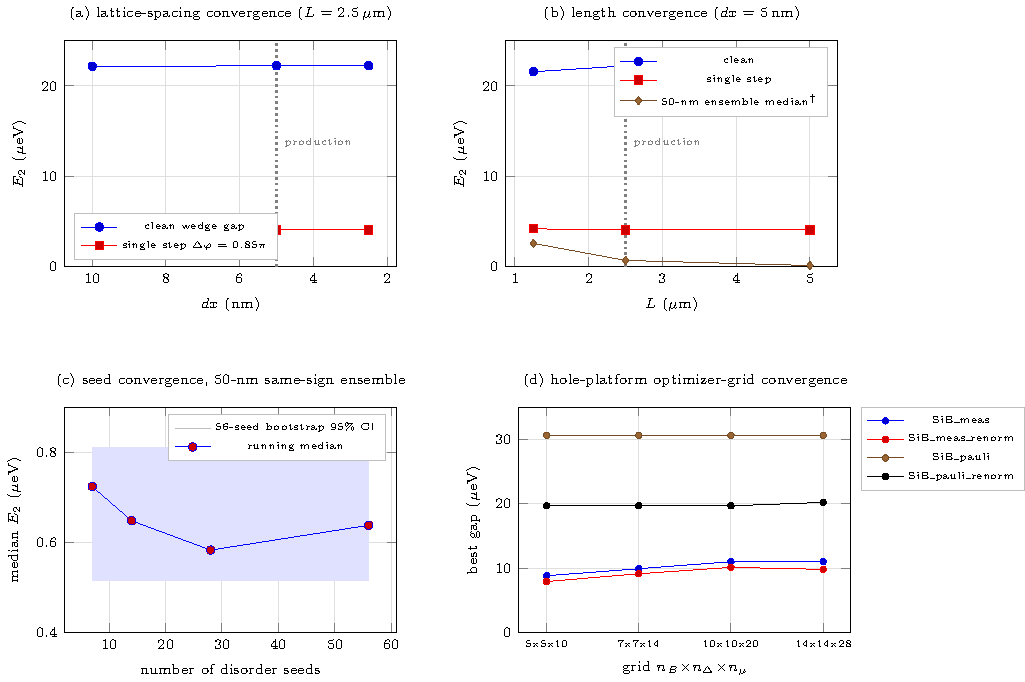
\includegraphics[width=\textwidth]{output/fig13_convergence.pdf}
\caption{Convergence summary (data: \texttt{convergence.json}; rendered by
\texttt{tools/fig13\_pgf.py}, equivalently \texttt{convergence.py} with
matplotlib). $^{\dagger}$The $L$-dependence of the step-ensemble median in
panel (b) is physical (Anderson localization), not a discretization artifact;
see Table~\ref{t:conv1}, note $a$.}
\label{f:conv}
\end{figure}

\section{Parent superconductor models and the $g=2$ optimum}\label{s:parent}
\subsection{What $\Delta$ is}
$\Delta$ in the BdG Hamiltonian is a \emph{static induced gap}: the
infinite-coupling limit of the standard tunneling self-energy
$\Sigma(\omega) = -\gamma\,(\omega + \Delta_p\tau_x)/\sqrt{\Delta_p^2 -
\omega^2}$ evaluated at $\omega = 0$, with
$\Delta_{ind} = \gamma\Delta_p/(\gamma + \Delta_p)$. We do not solve the
dynamical problem; instead (i) field suppression enters through the parent,
$\Delta_{ind} \le \Delta_p(B)$, with
$\Delta_p(B) = \Delta_0[1 - (B/B_c)^2]$ (GL, orbital-limited parents) or
$\Delta_0 - \mu_B B$ (Pauli-limited caricature), and (ii) metallization
enters through the quasiparticle weight $Z = 1 - \Delta_{ind}/\Delta_p$,
which renormalizes $\alpha \to Z\alpha$ and
$g \to Zg + (1-Z)g_p$ ($g_p = 2$). Both caricatures are stated wherever
used; replacing them by the full self-energy is listed as future work and
would \emph{lower} all gaps further (the renormalized numbers bound the
direction).

\subsection{Connection to Cole--Das Sarma--Stanescu}\label{s:cole}
Ref.~[Cole \emph{et al.}, PRB 92, 174511 (2015)] showed that strong
semiconductor--superconductor coupling buys induced-gap size at the price
of semiconductor properties ($g$, $\alpha$), so an intermediate coupling
optimizes the topological gap. Our $g=2$ ceiling is the sharp small-$g$
limit of that statement: with $E_Z(2\,\mathrm{T}) = 116\ueV$ fixed by
$g = 2$, the topological condition $E_Z > \sqrt{\Delta_{ind}^2 + \mu^2}$
cannot be met at all for $\Delta_{ind} \ge 116\ueV$, and maximizing the
gap over $(B, \Delta_{ind} \le \Delta_p(B), \mu)$ under GL suppression
yields an interior optimum $\Delta_0 \approx 98\ueV$
(main-text Sec.~3.2) --- i.e.\ for silicon electrons the Cole optimum is
not merely beneficial but \emph{mandatory}, and it caps the achievable
gap at a value disorder then destroys. The hole platform escapes through
$g_z$ up to 4.2, which moves the ceiling to $\sim 240\ueV$ at 2\,T.

\section{Quasiparticle-poisoning estimate}\label{s:qp}
The equilibrium quasiparticle fraction of the parent at temperature $T$ is
$x_{qp} \simeq \sqrt{2\pi k_BT/\Delta_p}\, e^{-\Delta_p/k_BT}$. Requiring
$x_{qp} \le 10^{-6}$ with the Si:B parent gap \emph{at the operating
field} ($\Delta_p(B^*) = 29$--$33\ueV$ for the measured-field design)
gives $T_{\mathrm{eff}} \le 25$--$29$\,mK; the same criterion for the Al
reference point of \texttt{qp\_poisoning.py} ($\Delta_p = 150\ueV$ at
$B = 1.0$\,T, GL) gives 130\,mK. Since realistic
electron temperatures in superconducting devices rarely reach 25\,mK,
the measured-field all-silicon stack is classified as a detection
platform (ZBP spectroscopy, gap hardness, the miscut test) rather than a
parity-coherent qubit, absent parent-gap engineering. All numbers in
\texttt{qp\_poisoning.py}.

\section{Luttinger--Kohn extraction}\label{s:lk}
The fin cross-section $(y,z)$ is solved in the 4-band LK Hamiltonian
(hard-wall, grid $11\times13$, $\gamma_1 = 4.285$, $\gamma_2 = 0.339$,
$\gamma_3 = 1.446$, $\kappa = -0.42$) with vertical field $E_z$; the
lowest Kramers doublet is followed in $k_x$ to extract $m^*$ (curvature),
$\alpha$ (linear-in-$k$ splitting), the SOC axis (spin direction of the
split states), and the $g$-tensor (bare $2\kappa\mu_B\mathbf{B\cdot J}$
plus orbital terms, evaluated as the field-derivative of the doublet
splitting along the three axes). Validation: at $E_z = 0$ the model
reproduces the exact bulk [100] heavy/light masses, and the predicted
spin--orbit lengths $l_{so} = \hbar^2/(m^*\alpha) = 32$--$101$\,nm overlap
the measured FinFET window ($\sim$20--60\,nm). Limits: no strain, no cubic ($J^3$) Zeeman, no
device electrostatics --- the known shortfall is $g_x \in [0.4, 1.1]$
across a seven-geometry bracket ($7$--$16$\,nm sections, 3--30\,MV/m)
versus measured $g_{xx} \approx 1.9$--$2.3$; all platform numbers are
therefore carried under both tensors, and the 6-band+Poisson resolution
is the top open theory item.

\section{Reproducibility}\label{s:repro}
Every figure and quoted number regenerates from the committed code:
\texttt{run\_analysis.py} (figures 1--11), \texttt{transport.py} /
\texttt{transport\_valley.py} (RGF, invariant, valley transport),
\texttt{lk\_holes.py}, \texttt{qp\_poisoning.py},
\texttt{convergence.py} (this supplement's Sec.~\ref{s:conv}),
\texttt{tests.py} (assertion suite covering the equivalence theorem,
gauge covariance, analytic dispersions, RGF agreement with closed-chain
spectra to $10^{-13}$, and regression tests for every bug found in
review). The numerical ledger is \texttt{output/data/key\_numbers.json};
scan checkpoints allow resuming every long run. Archival packaging
(commit hash, environment, per-figure commands) is described in
\texttt{README.md}; randomness is fully seeded (seed families are listed
in Tables~\ref{t:par-e}--\ref{t:par-h}).
\end{document}
